\chapter{The Application Infrastructure}

\section{System Architecture}

The Fake news detection system architecture is shown in\hyperref[fig:infrastructure]{Figure 3.1} it was inspired from balance transfer network [2]
 \begin{figure}[H]
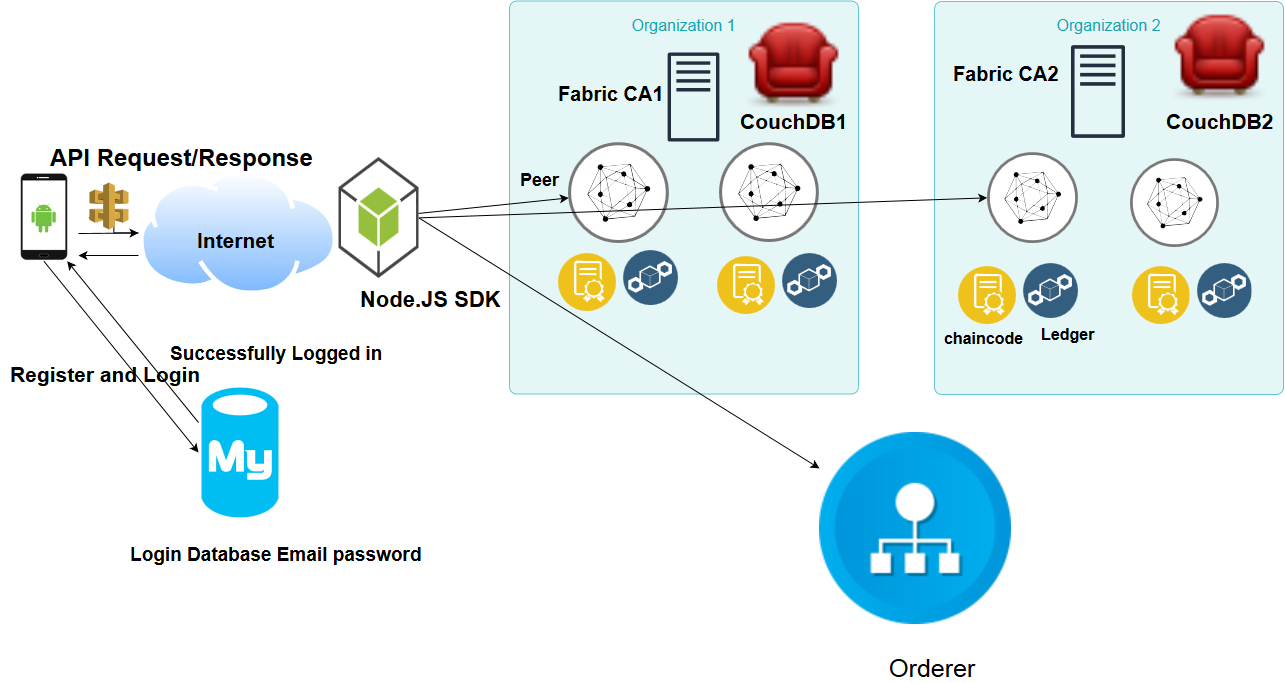
\includegraphics[width=15cm,height=12cm]{images/infrastructure.png}
\caption{The Application Infrastructure Overview}
\label{fig:infrastructure}
\end{figure}
\cleardoublepage

As shown, the system comprises of Two Organizations Organization 1 and organization 2. with two peers in each organization. 
With a solo orderer node.  There are also two fabric CA Server one for each organization, Two \textbf{Couch-DB} instances as world state for more efficient and rich queries. 
In addition, we are using node.js SDK  for interacting to the hyperledger fabric network and abstracting all the network infrastructure as a standard model thus the network could be scalable horizontally and vertically. All nodes are running on Docker containers for our testing purpose we implemented all the infrastructure on one Virtual Machine, However, in a production scenario every node should be an independent physical instance. \\ 

A layer of authentication using a traditional database was introduced so that the users could sign up on our application using the traditional way we used email and password, however integrating a phone authentication with One time pad could be a trivial thing. 
Once the user successfully login he could send requests from android device using our application to the SDK. and the SDK will handle the interaction with hyperledger fabric network and the chaincode. \\
 
The fabric CA Server will be responsible for Registration of identities, Issuance of Enrollment Certificates for signing and identifying, Issuance of Transaction Certificates and Providing both anonymity and unlinkability when transacting on a Hyperledger Fabric blockchain. All these functions are provided.
The network was the adoption of Balance transfer [2] A sample Node.js app to demonstrate fabric-client, fabric-ca-client, and Node.js SDK APIs. 
the main idea of the network is to demonstrate a simple use case app using hyperledger fabric in order to transfer a balance from a user to another one and query the chaincode. we modified the network, added a couch database instance and updating it with our chaincode. we modified the node.js application to suit our application. \\ 

Crypto material has been generated using the cryptogen tool from Hyperledger Fabric and mounted to all peers, the orderer node and CA containers. 
Beside An Orderer genesis block (genesis.block) and channel configuration transaction (mychannel.tx) has been pre-generated using the configtxgen tool from Hyperledger Fabric and placed within the artifacts folder. 

\section{Building the Network} 

Hyperledger Fabric came with many tools for facilitating the development process. As hyperledger fabric is modular by design many modules interacting together to make the application up and running.  
Once all prerequisites packages are installed on the platform where the application supposed to be installed. Hyperledger Fabric community provided fully annotated scripts that simply launches the network and generate the cryptographic material. \\ 

Initially, All the network topology should be pre-described in a yaml file, for instance, the number of organizations and peers, and the organization name. 
Taking into consideration that, every single operation must be signed and verified. as a result, every single network entities must have cryptographic materials (x509 certs and signing keys) those certificates will be used as identities and expedite the authentication process to take place as entities communicate and transact.  \\ 
One of those tools is Cryptogen tool which consumes the Yaml file describing the network and generates all required cryptographic materials, after running Cryptogen the generated certificates and keys will be saved to a folder titled crypto-config.

\clearpage 

\noindent \hyperref[fig:cryptoconfig]{Figure 3.2} describes the crypto config directory structure.  
 \begin{figure}[H]
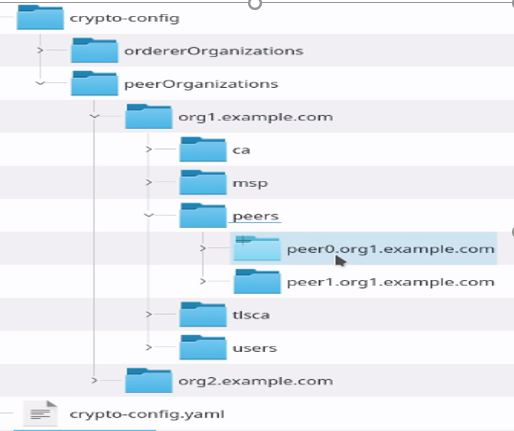
\includegraphics[width=15cm,height=12cm]{images/cryptoconfig.jpg}
\caption{Crypto Config Directory structure}
\label{fig:cryptoconfig}
\end{figure}


\noindent Configtxgen is used to generate the main configuration artifacts. such as genesis block, the channel and the anchor peers. 
Finally, docker-compose will be used to spin up the network. 

\section{Node.js App Backend and Node.js Fabric SDK} 
In our application we adopted one of the sample network provided by hyperledger fabric called balance transfer as a backend, this was done after modifying the main scripts to cope with our application requirements. 
\textbf{Balance Transfer} is a simple network with nodejs app that demonstrates fabric-client, fabric-ca-client, and Node.js SDK APIs.
\begin{itemize}
  \item Allows the communication with the hyperledger fabric network by using fabric node.js Libraries.
  \item Allows different operations using GET/POST requests, such as channel’s creation, joining the channel, installing and instantiating the chaincode.  
\end{itemize} 
\bigskip
\textbf{Node.js Fabrik SDK:} [3] eases the communication with hyperledger fabric blockchain using APIs. 
The Hyperledger Fabric SDK allows the interaction with the network on behalf of the users by simply calling APIs the following operations are supported: \\  

\begin{itemize}
   \item Creating channels.
   \item Allowing peers to join channels. 
   \item Installing chaincodes in the peers.
   \item Instantiating chaincodes in the a channel. 
   \item Querying the ledger. 
   \item Invoking transactions. 
\end{itemize}  
\bigskip
We used two main modules provided by the SDK: 

 \begin{itemize}
  \item fabric-client: Provides APIs to interact with the core components of a Hypreledger Fabric-based blockchain network, namely the peers, orderers and event streams.
  \item fabric-ca-client: Provides APIs to interact with the optional component, fabric-ca, that contains services for membership management.
\end{itemize} 
\bigskip

\section{Understanding Node.js APP} 
Node.js App[4] comprises of java scripts which simplify the process of the communication with hyperledger fabric network. it obscures all the network and exposes REST APIs for communication. the main files are highlighted as below. 
\ \\ 
\textbf{app.js} will route the requests in a modular way by avoiding the repetitive tasks. express node.js framework used to do all of those functionality. 
\ \\ 
\textbf{users.js} will validate if the user enrolled on the organization or not. If not it will enroll the user by calling fabric-ca-client and generate json web token JWT and returned top the user to make subsequent requests . 
\ \\ 
\textbf{helper.js} will load the network configuration settings, where all the keys are stored, thus the fabric-ca library could interact with the different hyperledger fabric entity. Furthermore, it will check if the user enrolled if not it will enroll by loading admin credentials and calling fabric-ca-client to enroll the user.
\ \\ 
\textbf{install-chaincode.js} contains the method for calling fabirc-client to install the chaincode on the peers.  \\ 
\ \\ 
\textbf{instantiate-chaincode.js} contains methods to instantiate the chaincode on the channel.  \\ 
\ \\  
\textbf{invoke-transaction.js} will invoke transaction proposals. \\
\ \\

\subsection{ Json Web Token(JWT) }
For securing the requests a jwt which is a signed token and returned to the application user.
Subsequently, the token can be sent over to the http request for every other request that needs authentication on the blockchain. \\ 
The application then validates the token and, if it’s valid, returns the secure resource to the client.
As per the below code snippet, the jwt will be expired after 10 hours then the user has to renew the jwt. \\ 

\begin{lstlisting}[language=Python, caption=JWT Generation]
const token = jwt.sign({
    exp: Math.floor(Date.now() / 1000) + parseInt(
        hfc.getConfigSetting('jwt_expiretime'), 10),
    username,
    orgName
}, app.get('secret'));

const response = await helper.getRegisteredUsers(username, orgName);

if (response && typeof response !== 'string') {
    res.json({
        success: true,
        token
    });
} else {
    res.json({
        success: false,
        message: response
    });
}
\end{lstlisting}
\cleardoublepage


\subsection{runApp.sh Script }
Using runApp.sh will spin up the network and expose the url all docker containers will be up and running. In addition, it will launch an instance of the app listening on port 4000. \\
\hyperref[fig:runapp]{Figure 3.3} displays simple output after running runApp.sh script. 
\ \\
 \begin{figure}[H]
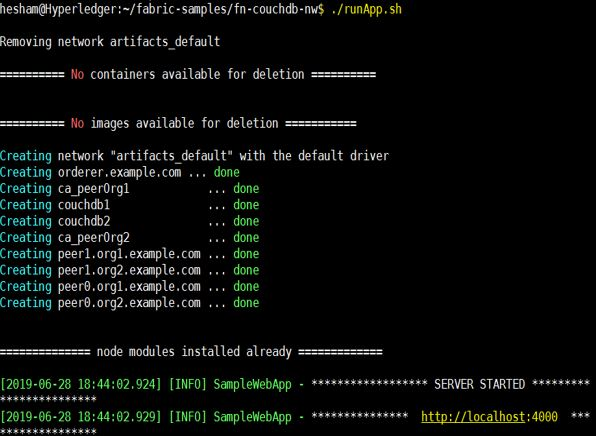
\includegraphics[width=15cm,height=12cm]{images/runapp.jpg}
\caption{runapp.sh Script Simple Output}
\label{fig:runapp}
\end{figure}


\subsection{testApi.sh Script }

After runApp.sh script successfully run and all network components are up and running. testApi.sh script will be responsible for creating a channel, allowing peers to join the channel, installing chaincode on the peers. last but not least instantiating the chaincode on the channel.
\cleardoublepage

\section{Mysql Login Database} 
In order to allow the application users to register to our application on a traditional way using email and password. We created a traditional relational MySQL database called "fake news" to store the users' email and hashed password with one table "login". 
We are making the process of users' registration independent from the blockchain network.
Although, We have only one server that hosts both the Xampp server and the fabric network. However, this is only for the development purpose. \\
\ \\ 
We created a simple XAMP Server consists of: 
\begin{itemize}
   \item Mysql Database: to store the login data information. 
   \item Apache as a webserver to serve the requests over the network. 
   \item Php as a scripting language to consume the requests and making different CRUD(Create, Update, Read, Delete) actions on the database.
   \item PhpMyadmin for simplifying the management of the database using a web interface. 
\end{itemize}  
\bigskip
The User will send a registration request using an email and password from the android device.  The request will be sent over the network, the Apache server is listening on port 80. We are calling register.php script for registering users. The register.php script check if the email already existed if not it will insert a record in the login table with the user email and the hashed password. and return the success response to the android as a confirmation. 
Similarly,  the login procedures, the user will send a login request using his email and hashed password by calling login.php. \\ 
\hyperref[fig:xampp]{Figure 3.4} describes the simple Xampp server and the fakenews database schema.     
 \begin{figure}[H]
\centering
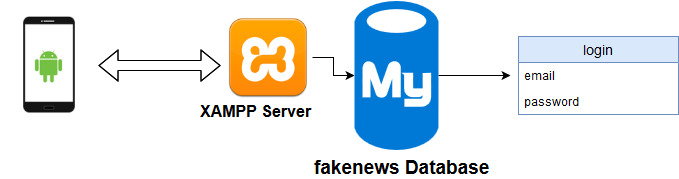
\includegraphics[width=10cm,height=5cm]{images/xampp.jpg}
\caption{Xampp Server Overview}
\label{fig:xampp}
\end{figure}

\cleardoublepage

\section{The Enrollment Procedures} 
This section describes the enrollment procedures as the following: 


\begin{enumerate}
  \item The user Will Register and login to the application using Email and password.
  \item Once the user successfully logged-in the application will send an enrollment request to the SDK using the user's email.
  \item The SDK forwards the enrollment Request to the Fabric-ca.
  \item Fabric-Ca generates the required ecerts and keys for the user and enrolls the user on the network.
   \item Once the user enrolled successfully the SDK generates JWT for the user and sends it to the application. 
    \item Finally, The application stores the JWT on the android device and includes it on the subsequent requests' header.
 
\end{enumerate}

\hyperref[fig:enrollmentproc]{Figure 3.5} depicts the whole operation.  
\ \\
 \begin{figure}[H]
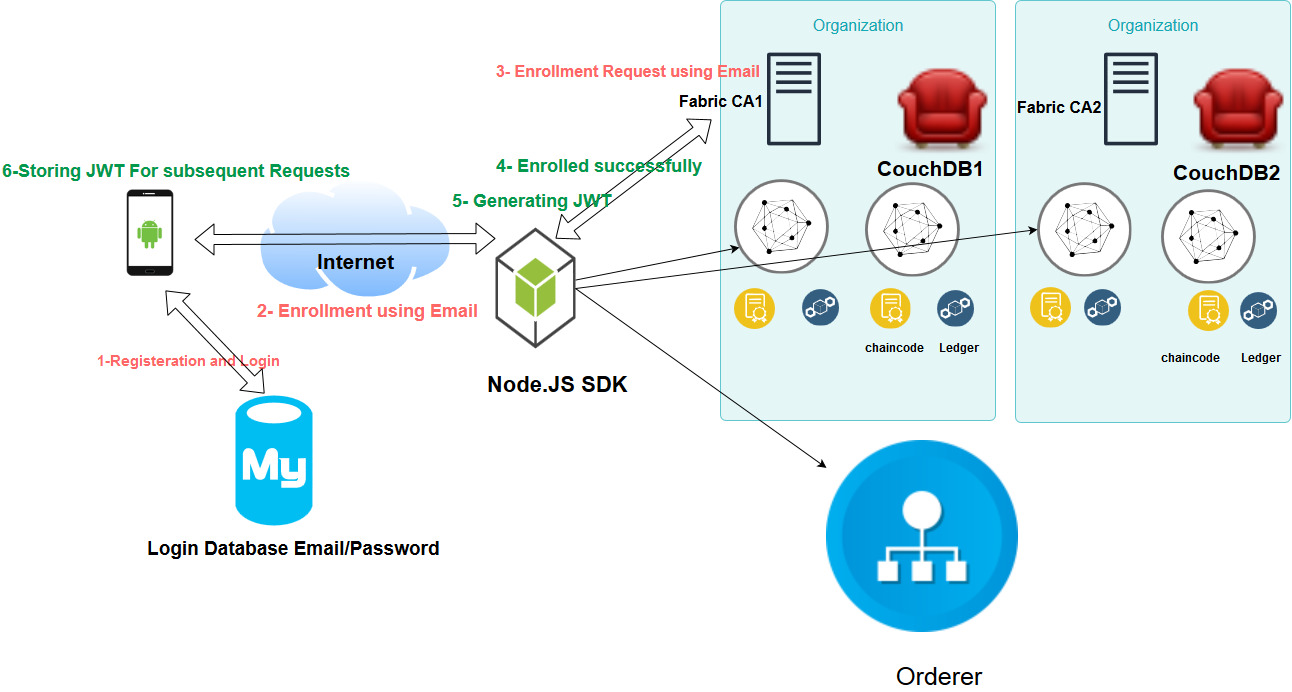
\includegraphics[width=15cm,height=12cm]{images/enrollmentproc.jpg}
\caption{The Enrollment Procedures}
\label{fig:enrollmentproc}
\end{figure}

  
\section{Calling The Rest API}

The node.js App obscuring the hyperledger fabric network and exposes a rest API endpoint to call, this will allow the application users to do different operations on the network. 
The application users could send a request by calling the URL endpoint using Post or Get Methods and passing the parameters, for instance, the chaincode name and arguments. In addition, JWT must be included in the request header. Once the request is made and sent over the internet the node.js app receives the request and forward it to SDK to make different operations on the ledger like invoke transactions or query the ledger. 
Once the transaction is made the response will be sent back to the Android application as a JSON response. The below listing illustrates an example of making an API call using curl command. calling the endpoint and attaching the JWT for authorization in the request header   

\begin{lstlisting}[caption={Simple REST API Call Using Curl},captionpos=b]
curl -s -X POST \
  http://localhost:4000/channels/mychannel/chaincodes/mycc \
  -H "authorization: Bearer $JWT" \
  -H "content-type: application/json" \
  -d '{
	"peers": ["peer0.org1.example.com","peer0.org2.example.com"],
	"fcn":"addEvent",
	"args":["{\"title\": \"foo\", \"location\": { \"latitude\": 52, \"longitude\": 10 }, \"description\": \"bar\" }"]
}'
\end{lstlisting}
\bigskip
The following Table shows the different functions provided by the chaincode for full API calls documnetation review [5]. \\  

\begin{tabular}{|p{4cm}|p{6cm}|p{3cm}|  }
\hline
\multicolumn{3}{|c|}{Chaincode API Calls} \\
\hline
CC Function name& Usage &Request Type \\
\hline
addEvent & Invoking an event to the chaincode & Post \\
queryEvents & Query The ledger & Get\\
 judgeEvent &Invoking an assessment on a specific events& Post \\
getFullEvent&Query a specific events with all it's assessments& Get\\
\hline
\end{tabular}







 








 



 
  